\documentclass{beamer}
\usepackage[english]{babel}
\usepackage[utf8]{inputenc}
\usepackage{verbatim}
\usepackage{graphicx}

\begin{document}

\title{Open Source Software: Easy to contribute}
\author{Maksim Melnikau (max\_posedon)}
\institute{Linux Mobile hobbyist\\World of Tanks developer}
\date{\today}
\frame{\titlepage}

\begin{frame}[fragile]{The Question}
    \begin{itemize}
        \pause \item How many of you opened at least one bug, which was fixed by upstream?
        \pause \item How many of you sent at least one patch, which was accepted by upstream?
        \pause \item Others, why are you don't contribute?
    \end{itemize}
\end{frame}

\begin{frame}[fragile]{Open Source waiting for you\alt<1>{}{r}}
    \begin{itemize}
        \pause
        \item mails
        \item documentation
        \item bugs
        \item patches
    \end{itemize}
\end{frame}

\begin{frame}[fragile]{It is easy and fun}
    \begin{figure}[htb]
    
\includegraphics[width=0.8\textwidth]{easy.jpg}
    \end{figure}
\end{frame}

\begin{frame}[fragile]{Take your favorite software\alt<1>{}{: systemd-cgtop}}
    \pause
    \begin{verbatim}
Path                                    Tasks   %CPU
/                                         477   27.0
/system                                     1   26.5
/system/kdm@.service                        -   25.2
/system/rabbitmq-server.service            44    0.7
/system/dbus.service                       12    0.3
/system/NetworkManager.service              4    0.2
/system/mysqld.service                     16    0.1
/system/avahi-daemon.service                2    0.0
/system/console-kit-daemon.service         65      -
/system/rtkit-daemon.service                3      -
/system/systemd-journald.service            1      -
/system/systemd-logind.service              1      -
/system/udev.service                        3      -
    \end{verbatim}
\end{frame}

\begin{frame}[fragile]{Bug 49778 - systemd-cgtop depth=3 better default than depth=2}
    \begin{figure}[htb]
        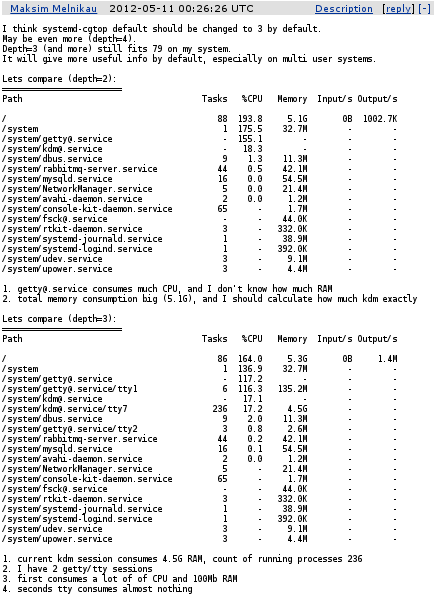
\includegraphics[width=0.5\textwidth]{bug.png}
    \end{figure}
\end{frame}

\begin{frame}[fragile]{Bug 49778 upstream fix}
    \begin{figure}[htb]
        
\includegraphics[width=1.0\textwidth]{comment.png}
    \end{figure}
    \begin{figure}[htb]
        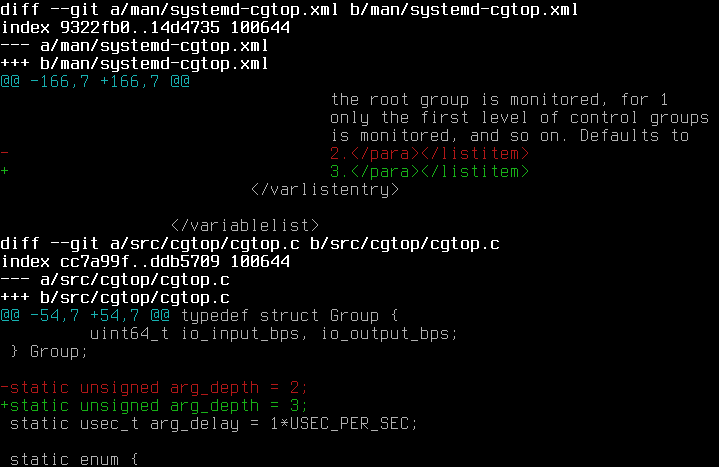
\includegraphics[width=1.0\textwidth]{fix.png}
    \end{figure}
\end{frame}

\begin{frame}[fragile]{systemd-cgtop --help}
\begin{verbatim}
systemd-cgtop [OPTIONS...]

Show top control groups by their resource usage.

  -h --help           Show this help
  --version           Print version and exit
  -p                  Order by path
  -t                  Order by number of tasks
  -c                  Order by CPU load
  -m                  Order by memory load
  -i                  Order by IO load
  -d --delay=DELAY    Specify delay
  -n --iterations=N   Run for N iterations before exiting
  -b --batch          Run in batch mode, accepting no input
     --depth=DEPTH    Maximum traversal depth (default: 2)
\end{verbatim}
\end{frame}

\begin{frame}[fragile]{patch}
    \begin{figure}[htb]
        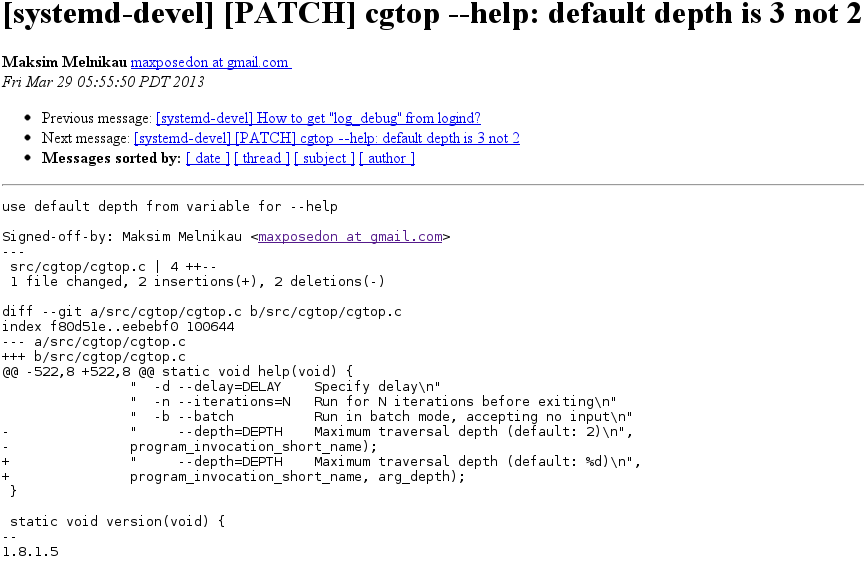
\includegraphics[width=1\textwidth]{patch.png}
    \end{figure}
\end{frame}

\begin{frame}[fragile]{apply}
    \begin{figure}[htb]
        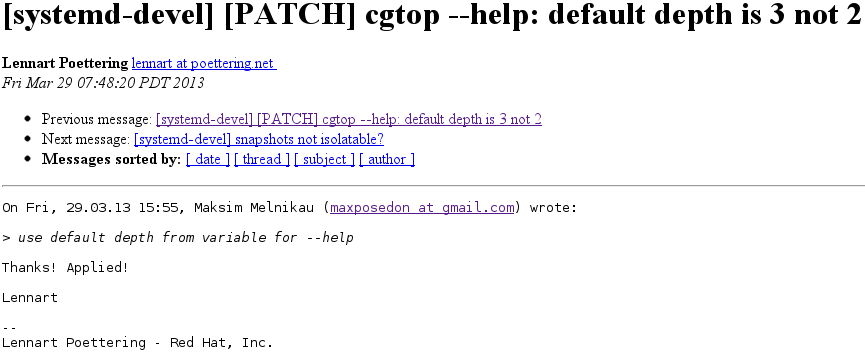
\includegraphics[width=1\textwidth]{apply.png}
    \end{figure}
\end{frame}

\begin{frame}[fragile]{Conclusion}
    Don't afraid - contribute! It's easy!
\end{frame}

\begin{frame}[fragile]{Ask me}
    \begin{itemize}
    \item \href{mailto:maxposedon@gmail.com}{maxposedon@gmail.com}
    \item \url{https://bugs.freedesktop.org/show\_bug.cgi?id=49778}
    \item \url{http://lists.freedesktop.org/archives/systemd-devel/2013-March/010005.html}
    \item \url{http://lists.freedesktop.org/archives/systemd-devel/2013-March/010009.html}
    \item \url{https://github.com/max-posedon/talk-easy-contribute}
    \end{itemize}
\end{frame}

\end{document}
